\documentclass[a4paper, 12pt]{article}

\usepackage{arxiv}

\usepackage[T2A]{fontenc}
\usepackage[utf8]{inputenc}
\usepackage[english, russian]{babel}
% \usepackage{cmap}
\usepackage{url}
\usepackage{booktabs}
\usepackage{nicefrac}
\usepackage{microtype}
\usepackage{lipsum}
\usepackage{graphicx}
\usepackage{epstopdf}
\usepackage{subfig}
\usepackage[square,sort,comma,numbers]{natbib}
\usepackage{doi}
\usepackage{multicol}
\usepackage{multirow}
\usepackage{tabularx}
\usepackage{float}

\usepackage{tikz}
\usetikzlibrary{matrix}

% Algorithms
\usepackage{algpseudocode}
\usepackage{algorithm}

%% Шрифты
\usepackage{euscript} % Шрифт Евклид
\usepackage{mathrsfs} % Красивый матшрифт
\usepackage{extsizes} % Возможность сделать 14-й шрифт
\usepackage{bm}

\usepackage{makecell} % diaghead in a table
\usepackage{amsmath,amsfonts,amssymb,amsthm,mathtools,dsfont}
\usepackage{icomma}
\usepackage[labelfont=bf]{caption}
\usepackage{subfig} % for subfigures
\usepackage{wrapfig}

\newcommand{\bz}{\mathbf{z}}
\newcommand{\bx}{\mathbf{x}}
\newcommand{\by}{\mathbf{y}}
\newcommand{\bv}{\mathbf{v}}
\newcommand{\bw}{\mathbf{w}}
\newcommand{\ba}{\mathbf{a}}
\newcommand{\bb}{\mathbf{b}}
\newcommand{\bp}{\mathbf{p}}
\newcommand{\bq}{\mathbf{q}}
\newcommand{\bt}{\mathbf{t}}
\newcommand{\bu}{\mathbf{u}}
\newcommand{\bs}{\mathbf{s}}
\newcommand{\bT}{\mathbf{T}}
\newcommand{\bX}{\mathbf{X}}
\newcommand{\bZ}{\mathbf{Z}}
\newcommand{\bS}{\mathbf{S}}
\newcommand{\bH}{\mathbf{H}}
\newcommand{\bW}{\mathbf{W}}
\newcommand{\bY}{\mathbf{Y}}
\newcommand{\bU}{\mathbf{U}}
\newcommand{\bQ}{\mathbf{Q}}
\newcommand{\bP}{\mathbf{P}}
\newcommand{\bA}{\mathbf{A}}
\newcommand{\bB}{\mathbf{B}}
\newcommand{\bC}{\mathbf{C}}
\newcommand{\bE}{\mathbf{E}}
\newcommand{\bF}{\mathbf{F}}
\newcommand{\bomega}{\boldsymbol{\omega}}
\newcommand{\btheta}{\boldsymbol{\theta}}
\newcommand{\bgamma}{\boldsymbol{\gamma}}
\newcommand{\bdelta}{\boldsymbol{\delta}}
\newcommand{\bPsi}{\boldsymbol{\Psi}}
\newcommand{\bpsi}{\boldsymbol{\psi}}
\newcommand{\bxi}{\boldsymbol{\xi}}
\newcommand{\bchi}{\boldsymbol{\chi}}
\newcommand{\bzeta}{\boldsymbol{\zeta}}
\newcommand{\blambda}{\boldsymbol{\lambda}}
\newcommand{\beps}{\boldsymbol{\varepsilon}}
\newcommand{\bZeta}{\boldsymbol{Z}}
% mathcal
\newcommand{\cX}{\mathcal{X}}
\newcommand{\cY}{\mathcal{Y}}
\newcommand{\cW}{\mathcal{W}}

\newcommand{\dH}{\mathds{H}}
\newcommand{\dR}{\mathds{R}}
% transpose
\newcommand{\T}{^{\mathsf{T}}}

% \renewcommand{\shorttitle}{\textit{arXiv} Шаблон}
\renewcommand{\epsilon}{\ensuremath{\varepsilon}}
\renewcommand{\phi}{\ensuremath{\varphi}}
\renewcommand{\kappa}{\ensuremath{\varkappa}}
\renewcommand{\le}{\ensuremath{\leqslant}}
\renewcommand{\leq}{\ensuremath{\leqslant}}
\renewcommand{\ge}{\ensuremath{\geqslant}}
\renewcommand{\geq}{\ensuremath{\geqslant}}
\renewcommand{\emptyset}{\varnothing}

\DeclareMathOperator*{\argmax}{arg\,max}  % in your preamble
\DeclareMathOperator*{\argmin}{arg\,min}  % in your preamble 

\usepackage{hyperref}
% \usepackage[usenames,dvipsnames,svgnames,table,rgb]{xcolor}

\hypersetup{
	unicode=true,
	colorlinks=true,
	linkcolor=black,        % внутренние ссылки
	citecolor=blue,         % на библиографию
	filecolor=magenta,      % на файлы
	urlcolor=blue           % на URL
}

\graphicspath{{./figures}}

\usepackage{enumitem} % Для модификаций перечневых окружений

\theoremstyle{definition} % "Определение"
\newtheorem{definition}{Опр.}[section]

\usepackage{etoolbox}

\makeatletter
\expandafter\patchcmd\csname\string\algorithmic\endcsname{\itemsep\z@}{\itemsep=1.5mm}{}{}
\makeatother

\newcommand{\myfigref}[2]{~\ref{#1}.\subref{#2}}% <---- a new macro for referring to a subfigure
\renewcommand{\abstractname}{Аннотация}

\title{Восстановление снимков фМРТ по просматриваемому видеоряду}

\author{
	%Дорин Даниил \\
	%\texttt{dorin.dd@phystech.edu} \\
	%\And
	Киселев Никита \\
	\texttt{kiselev.ns@phystech.edu} \\
	\And
	Грабовой Андрей \\
	\texttt{grabovoy.av@phystech.edu}
}
\date{\today}

\begin{document}
\maketitle

\begin{abstract}
	
	Исследуется проблема восстановления зависимости между показаниями датчиков фМРТ
	и восприятием внешнего мира человеком.
	Проводится анализ зависимости между последовательностью снимков фМРТ и видеорядом,
	просматриваемым человеком.
	На основе исследования зависимости предлагается метод аппроксимации показаний фМРТ по
	просматриваемому видеоряду.
	Для анализа предложенного метода проводится вычислительный эксперимент на 
	выборке, полученной при томографическом обследовании большого числа испытуемых.

\end{abstract}


\keywords{нейровизуализация \and фМРТ \and видеоряд \and зависимость между данными}

\section{Введение}

	Совокупность методов, визуализирующих структуру и функции человеческого мозга,
	называется \textit{нейровизуализацией}. Методы нейровизуализации, такие как ЭКГ, КТ, МРТ и фМРТ, 
	используются для изучения мозга, а также для обнаружения заболеваний и психических расстройств. 

	\textit{Функциональная магнитно-резонансная томография} или \textit{фМРТ} (англ.~\textit{fMRI}) 
	является разновидностью магнитно-резонансной томографии и основана на изменениях в токе крови, 
	вызванных нейронной активностью мозга \citep{Glover2011}. 
	Эти изменения происходят не моментально, а с некоторой задержкой.
	Она возникает из-за того, что сосудистая система достаточно долго реагирует 
	на потребность мозга в глюкозе \citep{Logothetis2003}. Изображения, получаемые с помощью фМРТ,
	показывают, какие участки мозга активированы при выполнении испытуемым определенных заданий.

	Настоящая работа посвящена восстановлению зависимости между снимками фМРТ и видеорядом.
	Используется предположение, что такая зависимость существует.
	Кроме того, предполагается, что между снимком и видеорядом есть постоянная задержка во времени
	\citep{Logothetis2003}.
	Проверяется зависимость снимка фМРТ от одного изображения.
	Время задержки выступает в качестве гиперпараметра модели.
	На основе анализа зависимости предлагается метод аппроксимации показаний фМРТ по
	просматриваемому видеоряду.

	Метод фМРТ играет большую роль в нейровизуализации, однако имеет ряд важных ограничений.
	В работах \citep{menon1999spatial, logothetis2008we} рассматриваются 
	временное и пространственное разрешения фМРТ. Временное разрешение является существенным
	недостатком данного метода. Другой недостаток фМРТ~--- неизбежно возникающие шумы, 
	связанные с движением объекта в сканере, сердцебиением и дыханием человека, тепловыми
	флуктуациями самого прибора и т.\,д. В работе \citep{1804.10167} предлагаются методы 
	подавления вышеперечисленных шумов на основе графов и демонстрируется их эффективность в задаче
	выявления эпилепсии и депрессии.

	Обобщением уже естественных для обработки изображений 2D сверток в CNN являются 3D
	свертки \citep{Tran_2015_ICCV}.
	Они агрегируют информацию как по времени, так и по пространству.
	Однако это приводит к сильному увеличению количества используемых параметров.
	В~настоящей работе используется наиболее современная архитектура~--- Transformer.
	Впервые она была предложена в статье \citep{https://doi.org/10.48550/arxiv.1706.03762}.
	Не так давно появилась адаптация архитектуры Transformer для работы с видео
	\citep{https://doi.org/10.48550/arxiv.2201.04288}. Данная архитектура состоит из кодировщика
	и декодировщика, каждый из которых в свою очередь состоит из отдельных слоев. Использование 
	механизма Attention \citep{https://doi.org/10.48550/arxiv.1706.03762} 
	позволяет значительно повысить качество работы модели.

	Данные, на которых проводятся проверка гипотезы зависимости и демонстрация работы построенного 
	метода, представлены в работе \citep{Berezutskaya2022}. Этот набор данных был получен при
	обследовании группы из 63 испытуемых. Тридцать из них проходили обследование фМРТ.
	Им предлагалось выполнить одно и то же задание~--- просмотреть короткий аудиовизуальный фильм. 
	Для него в рассматриваемой работе были сгенерированы аннотации, содержащие в том числе информацию о времени появления и исчезновения
	отдельных слов, объектов и персонажей. Методы аудио- и видеоаннотирования подробно излагаются в
	\citep{boersma2018praat} и \citep{Berezutskaya2020}. 

\section{Постановка задачи}

	Задана частота кадров $\nu \in \mathbb{R}$ и продолжительность $t \in \mathbb{R}$ видеоряда. 
	Задан видеоряд
	\begin{equation}
		\label{eq1}
		\bP = [\bp_1, \ldots, \bp_{\nu \cdot t}], \quad\
		\bp_i \in \mathbb{R}^{W_{\bP} \times H_{\bP} \times C_{\bP}},
	\end{equation}
	с шириной, высотой и числом каналов изображения $W_{\bP}, H_{\bP}$ и 
	$C_{\bP}$ соответственно.

	Обозначим частоту снимков фМРТ $\mu \in \mathbb{R}$. Задана последовательность снимков 
	\begin{equation}
		\label{eq2}
		\bS = [\bs_1, \ldots, \bs_{\mu \cdot t}], \quad\
		\bs_i \in \mathbb{R}^{W_{\bS} \times H_{\bS} \times D_{\bS}},
	\end{equation}
	где $W_{\bS}, H_{\bS}$ и $D_{\bS}$~--- размерности воксельного изображения. 

	Задача состоит в построении отображения, которое бы учитывало задержку $\Delta t$ между
	снимком фМРТ и видеорядом, а также предыдущие томографические показания. Формально, необходимо
	найти такое отображение $g$, что
	\begin{equation}
		\label{eq3}
		g(\bp_1, \ldots, \bp_{k_i - \nu \cdot \Delta t}; \bs_1, \ldots, \bs_{i-1}) = \bs_i,
		\ i = 1, \ldots, \mu t,
	\end{equation}
	где для $i$-го снимка фМРТ номер соответствующего изображения $k_i$ определяется по формуле
	\begin{equation}
		\label{eq4}
		k_i = \dfrac{i \cdot \nu}{\mu}.
	\end{equation}

\section{Вычислительный эксперимент}

\subsection{Цель эксперимента}

	Целью вычислительного эксперимента является выбор оптимального метода аппроксимации
	отображения \eqref{eq3}. Данные для эксперимента взяты из работы \citep{Berezutskaya2022}. 
	Набор данных содержит результаты обследования 63 испытуемых. Для тридцати из них известны
	показания фМРТ.

	Последовательность снимков для испытуемого представляется в виде тензора.
	Каждый снимок представляется тензором третьего ранга с размерностями 
	\[ W_{\bS} = 40, H_{\bS} = 64, D_{\bS} = 64. \]
	Частота снимков $\mu = 1,64$ кадров в секунду, продолжительность $t = 390$~с, 
	число снимков $N_{\bS} = \mu \cdot t = 641$. Таким образом, 
	\[ \bS = [\bs_1, \ldots, \bs_{641}] \in \mathbb{R}^{40 \times 64 \times 64 \times 641}. \]

	Продолжительность видео также $t = 390$~c, частота кадров $\nu = 25$, число изображений
	$N_{\bP} = \nu \cdot t = 9750$.
	Каждое изображение представляется в виде тензора третьего ранга с размерностями
	\[ W_{\bP} = 640, H_{\bP} = 480, C_{\bP} = 3. \]
	Тензор видеоряда
	\[ \bP = [\bp_1, \ldots, \bp_{9750}] \in \mathbb{R}^{640 \times 480 \times 3 \times 9750}. \]

	Согласно \eqref{eq4}, номер изображения, соответствующего снимку фМРТ, $k_i = 15 \cdot i$.
	Тогда суммарное число пар (изображение, снимок) равно $N = N_{\bS} - \mu \Delta t = 641 - \mu \Delta t$.

\subsection{Базовый метод}

	Предположим, что каждый снимок фМРТ зависит только от одного изображения. Тогда соответствующее
	отображение
	\begin{equation}
		\label{eq5}
		g(\bp_{k_i - \nu \cdot \Delta t}) = \bs_i, \ i = 1, \ldots, \mu t.
	\end{equation}

	Рассмотрим снимок $\bs_{\ell} = [v^{\ell}_{ijk}] \in \mathbb{R}^{40 \times 64 \times 64}$,
	где $v^{\ell}_{ijk} \in \mathbb{R}_+$~--- значение соответствующего вокселя.
	Для каждого изображения из видеоряда был получен вектор признакового описания
	размерности $d = 2048$:
	\[ \bx_i = [x^i_1, \ldots, x^i_{d}]\T \in \mathbb{R}^{d}, \ i = 1, \ldots, 9750. \]
	Использовалась архитектура нейронной сети ResNet152 без последнего линейного слоя.
	
	Таким образом, для каждого вокселя задана выборка
	\[ \mathfrak{D}_{ijk} = \{(\bx_{\ell}, v^{\ell}_{ijk}) \ | \ {\ell} = 1, \ldots, N \}. \]

	Поставлена задача восстановления регрессии
	\begin{equation}
		\label{eq6}
		y_{ijk}: \mathbb{R}^{d} \to \mathbb{R}.
	\end{equation}
	
	Используется линейная модель с вектором параметров 
	\[ \bw_{ijk} = [w^{ijk}_1, \ldots, w^{ijk}_{d}]\T \in \mathbb{R}^{d}: \]
	\begin{equation}
		\label{eq7}
		f_{ijk}(\bx, \bw_{ijk}) = \langle \bx, \bw_{ijk} \rangle.
	\end{equation}

	Для модели $f_{ijk}$ с соответствующим ей вектором параметров $\bw_{ijk} \in \mathbb{R}^{d}$
	определим квадратичную функцию потерь:
	\begin{equation}
		\label{eq8}
		\mathcal{L}_{ijk}(\bw_{ijk}, \Delta t) = \sum\limits_{\ell = 1}^{N_{\bS} - \mu \Delta t} \big(f_{ijk}(\bx_{\ell}, \bw_{ijk}) - v^{\ell}_{ijk}\big)^2.
	\end{equation}

	Требуется найти параметры, доставляющие минимум функционалу потерь $\mathcal{L}_{ijk}(\bw_{ijk}, \Delta t)$
	при заданном гиперпараметре $\Delta t$:
	\begin{equation}
		\label{eq9}
		\hat{\bw}_{ijk} = \argmin_{\bw_{ijk}} \mathcal{L}_{ijk}(\bw_{ijk}, \Delta t).
	\end{equation}

	Минимум функции потерь находится методом наименьших квадратов. Определим матрицу плана
	\begin{equation}
		\label{eq10}
		\bX = [\bx_1\T, \ldots, \bx_N\T]\T = [x^i_j] \in \mathbb{R}^{N \times d}
	\end{equation}
	и вектор, компонентами которого являются значения одного и того же вокселя в разных снимках,
	\begin{equation}
		\label{eq11}
		\bv_{ijk} = [v^1_{ijk}, \ldots, v^N_{ijk}]\T \in \mathbb{R}^N.
	\end{equation}
	Решение можно записать в виде
	\begin{equation}
		\label{eq12}
		\hat{\bw}_{ijk} = (\bX\T \bX)^{-1} \bX\T \bv_{ijk} = \bX^{+} \bv_{ijk},
	\end{equation}
	где $\bX^{+}$~--- псевдообратная матрица для $\bX$.
	
	Получим формулу для восстановленных снимков фМРТ. Введем матрицу весов
	\begin{equation}
		\label{eq13}
		\bW = [\bw_1\T, \ldots, \bw_{W_{\bS} \cdot H_{\bS} \cdot D_{\bS}}\T]\T = [w^i_j] \in \mathbb{R}^{W_{\bS} \cdot H_{\bS} \cdot D_{\bS} \times d}.
	\end{equation}
	Тогда строки матрицы
	\begin{equation}
		\label{eq14}
		\bX \cdot \bW\T = [\hat{v}^{\ell}_{ijk}] \in \mathbb{R}^{N \times W_{\bS} \cdot H_{\bS} \cdot D_{\bS}}
	\end{equation}
	содержат значения вокселей соответствующего снимка. После преобразования каждой строки в тензор 
	третьего ранга получаем восстановленный снимок $\hat{\bs}_{\ell}$.

	Размерность снимка фМРТ предварительно понижается с помощью сверточного слоя MaxPool3D.
	Рассматриваются коэффициенты сжатия 1, 2, 4 и 8.
	Значения вокселей нормализуются процедурой MinMaxScale.
	Производится разделение выборки на обучающую и тестовую.
	Качество рассматриваемого метода оценивается с помощью метрики MSE.
	Усреднение берется по всем снимкам фМРТ в тестовой выборке и по всем вокселям снимка.

\subsubsection{Предварительные результаты}

	Проанализирована зависимость качества восстановления снимков фМРТ от гиперпараметра $\Delta t$.
	Использовалось предварительное 8-кратное сжатие снимка.
	Зависимость метрики MSE от гиперпараметра $\Delta t$ представлена на Рис.~\ref{fig:2}.

	На Рис.~\ref*{fig:1} представлены срезы истинного и восстановленного снимков из 
	тестовой выборки. На Рис.\myfigref{fig:1}{fig:1c} можно наблюдать восстановленный снимок, к 
	которому была применена операция отсечения нефизичных значений и применен фильтр Гаусса.
	Использовалось оптимальное значение $\Delta t = 4 \text{ с}$.

	\begin{figure}[h!]
		\centering
		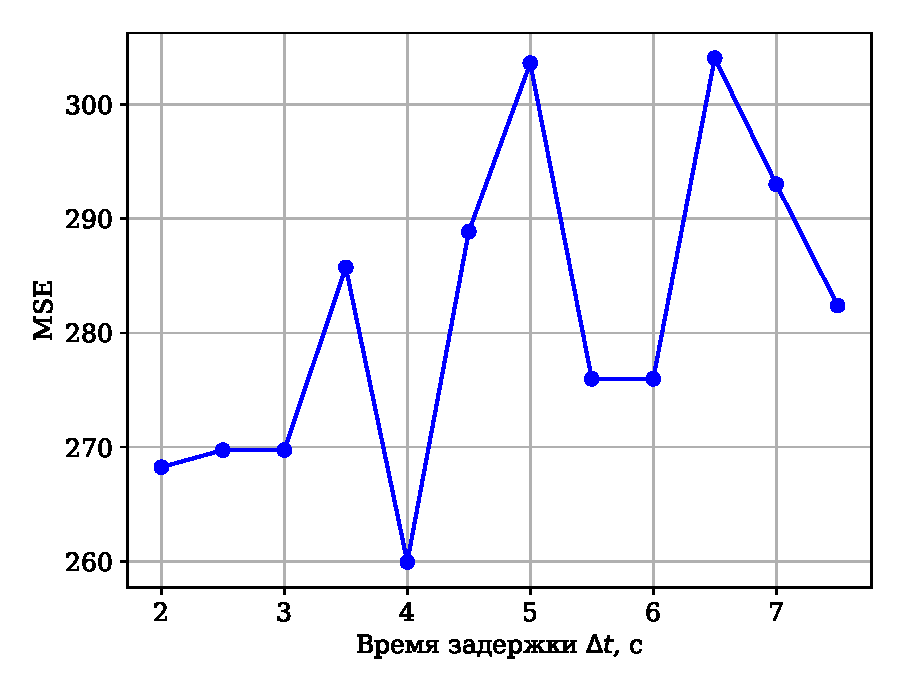
\includegraphics[width=0.65\textwidth]{MSE_dt.eps}
		\caption{Зависимость метрики MSE от гиперпараметра $\Delta t$ на снимке из тестовой выборки}
		\label{fig:2}
	\end{figure}

	\begin{figure}[h!]
		\centering
		\subfloat[Истинный]{\label{fig:1a}{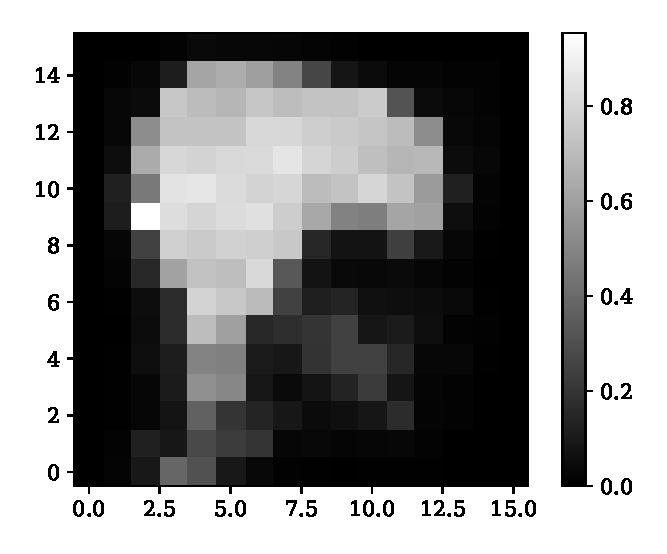
\includegraphics[width=0.33\textwidth]{sub-04-4-4-5-_-_-orig.eps}}}
		\hfill
		\subfloat[Восстановленный]{\label{fig:1b}{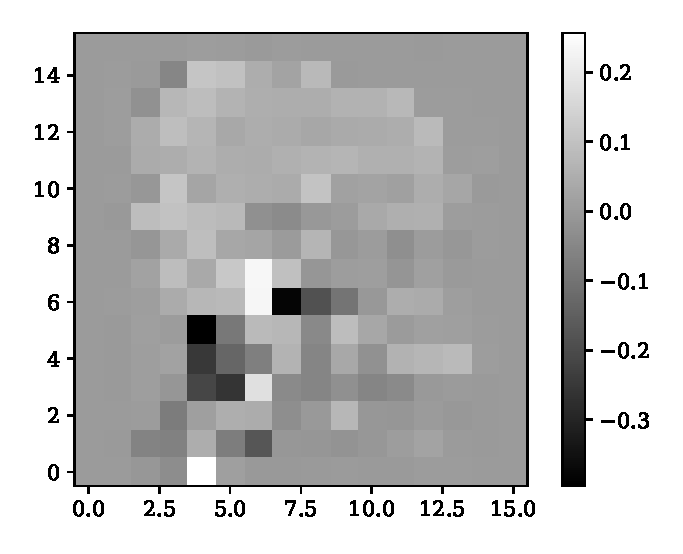
\includegraphics[width=0.33\textwidth]{sub-04-4-4-5-_-_-pred.eps}}}
		\hfill
		\subfloat[Обработанный]{\label{fig:1c}{\includegraphics[width=0.33\textwidth]{sub-04-4-4-5-_-_-pred-pg.eps}}}
		\caption{Срез снимка фМРТ из тестовой выборки}
		\label{fig:1}
	\end{figure}
	
	В рассматриваемом методе не учитывается зависимость значений соседних вокселей.
	Это является его главным недостатком, что приводит к большим выбросам в восстановленных снимках
	и малой контрастности. Несмотря на это, на восстановленных снимках отчетливо видны границы
	активных областей.

\subsection{Основной метод}

	Предположим, что каждый снимок фМРТ зависит только от одного изображения и предыдущего снимка.
	Тогда соответствующее отображение
	\begin{equation}
		\label{eq15}
		g(\bp_{k_i - \nu \Delta t}; \bs_{i-1}) = \bs_i, \ i = 1, \ldots, \mu t.
	\end{equation}

	Аналогично базовому методу, для каждого вокселя задана выборка
	\[ \mathfrak{D}_{ijk} = \{(\bx_{\ell}, v^{\ell + 1}_{ijk} - v^{\ell}_{ijk}) \ | \ {\ell} = 1, \ldots, N-1 \}. \]

	Используется такая же линейная модель. Добавляется слагаемое $L_2$-регуляризации. 
	Квадратичная функция потерь принимает вид
	\begin{equation}
		\label{eq16}
		\mathcal{L}_{ijk}(\bw_{ijk}, \Delta t) = \sum\limits_{\ell = 1}^{N_{\bS} - \mu \Delta t - 1} \big(f_{ijk}(\bx_{\ell}, \bw_{ijk}) - (v^{\ell + 1}_{ijk} - v^{\ell}_{ijk})\big)^2 + \alpha \| \bw_{ijk} \|_2^2.
	\end{equation}

	Вновь требуется найти параметры, доставляющие минимум функционалу потерь $\mathcal{L}_{ijk}(\bw_{ijk}, \Delta t)$
	при заданном гиперпараметре $\Delta t$:
	\begin{equation}
		\label{eq17}
		\hat{\bw}_{ijk} = \argmin_{\bw_{ijk}} \mathcal{L}_{ijk}(\bw_{ijk}, \Delta t).
	\end{equation}

	Минимум функции потерь находится методом наименьших квадратов. Определим матрицу плана
	\begin{equation}
		\label{eq18}
		\bX = [\bx_2\T, \ldots, \bx_N\T]\T = [x^i_j] \in \mathbb{R}^{(N-1) \times d}
	\end{equation}
	и вектор, компонентами которого являются разности значений одного и того же вокселя в разных снимках,
	\begin{equation}
		\label{eq19}
		\mathbf{\Delta v}_{ijk} = [v^2_{ijk} - v^1_{ijk}, \ldots, v^N_{ijk} - v^{N-1}_{ijk}]\T \in \mathbb{R}^{N-1}.
	\end{equation}
	Решение можно записать в виде
	\begin{equation}
		\label{eq20}
		\hat{\bw}_{ijk} = (\bX\T \bX + \alpha \mathbf{I})^{-1} \bX\T \mathbf{\Delta v}_{ijk}.
	\end{equation}

	Получим формулу для восстановленных снимков фМРТ. Введем матрицу весов
	\begin{equation}
		\label{eq21}
		\bW = [\bw_1\T, \ldots, \bw_{W_{\bS} \cdot H_{\bS} \cdot D_{\bS}}\T]\T = [w^i_j] \in \mathbb{R}^{W_{\bS} \cdot H_{\bS} \cdot D_{\bS} \times d}.
	\end{equation}
	Тогда строки матрицы
	\begin{equation}
		\label{eq22}
		\bX \cdot \bW\T = [\hat{v}^{\ell+1}_{ijk} - \hat{v}^{\ell}_{ijk}] \in \mathbb{R}^{(N-1) \times W_{\bS} \cdot H_{\bS} \cdot D_{\bS}}
	\end{equation}
	содержат разности значений вокселей двух последовательных снимков. 
	
	К получившейся матрице прибавим матрицу
	\begin{equation}
		\label{eq23}
		[v^{\ell}_{ijk}] \in \mathbb{R}^{(N-1) \times W_{\bS} \cdot H_{\bS} \cdot D_{\bS}}.
	\end{equation}
	
	После преобразования каждой строки в тензор третьего ранга получаем восстановленный снимок $\hat{\bs}_{\ell}$.

	Размерность снимка фМРТ предварительно понижается с помощью сверточного слоя MaxPool3D.
	Рассматриваются коэффициенты сжатия 1, 2, 4 и 8.
	Значения вокселей нормализуются процедурой MinMaxScale.
	Производится разделение выборки на обучающую и тестовую.
	Качество рассматриваемого метода оценивается с помощью метрики MSE.
	Усреднение берется по всем снимкам фМРТ в тестовой выборке и по всем вокселям снимка.

\section{Анализ ошибки}

	Проанализирована зависимость качества восстановления снимков фМРТ от гиперпараметра $\Delta t$.
	Использовалось предварительное 8-кратное сжатие снимка.
	Зависимость метрики MSE от гиперпараметра $\Delta t$ представлена на Рис.~\ref{fig:3}.

	\begin{figure}[h!]
		\centering
		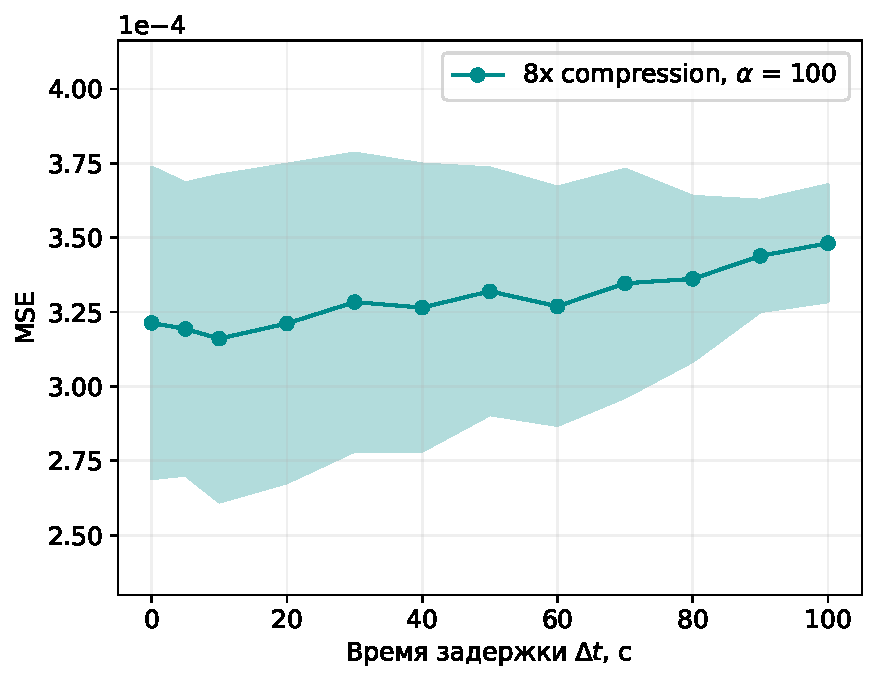
\includegraphics[width=0.65\textwidth]{subs_delta_MSE_dt.pdf}
		\caption{Зависимость метрики MSE от гиперпараметра $\Delta t$ на снимках из тестовой выборки}
		\label{fig:3}
	\end{figure}

	На Рис.~\ref*{fig:4} представлены срезы истинного и восстановленного снимков из 
	тестовой выборки. На Рис.\myfigref{fig:4}{fig:4c} можно наблюдать разность между ними.

	\begin{figure}[h!]
		\centering
		\subfloat[Истинный]{\label{fig:4a}{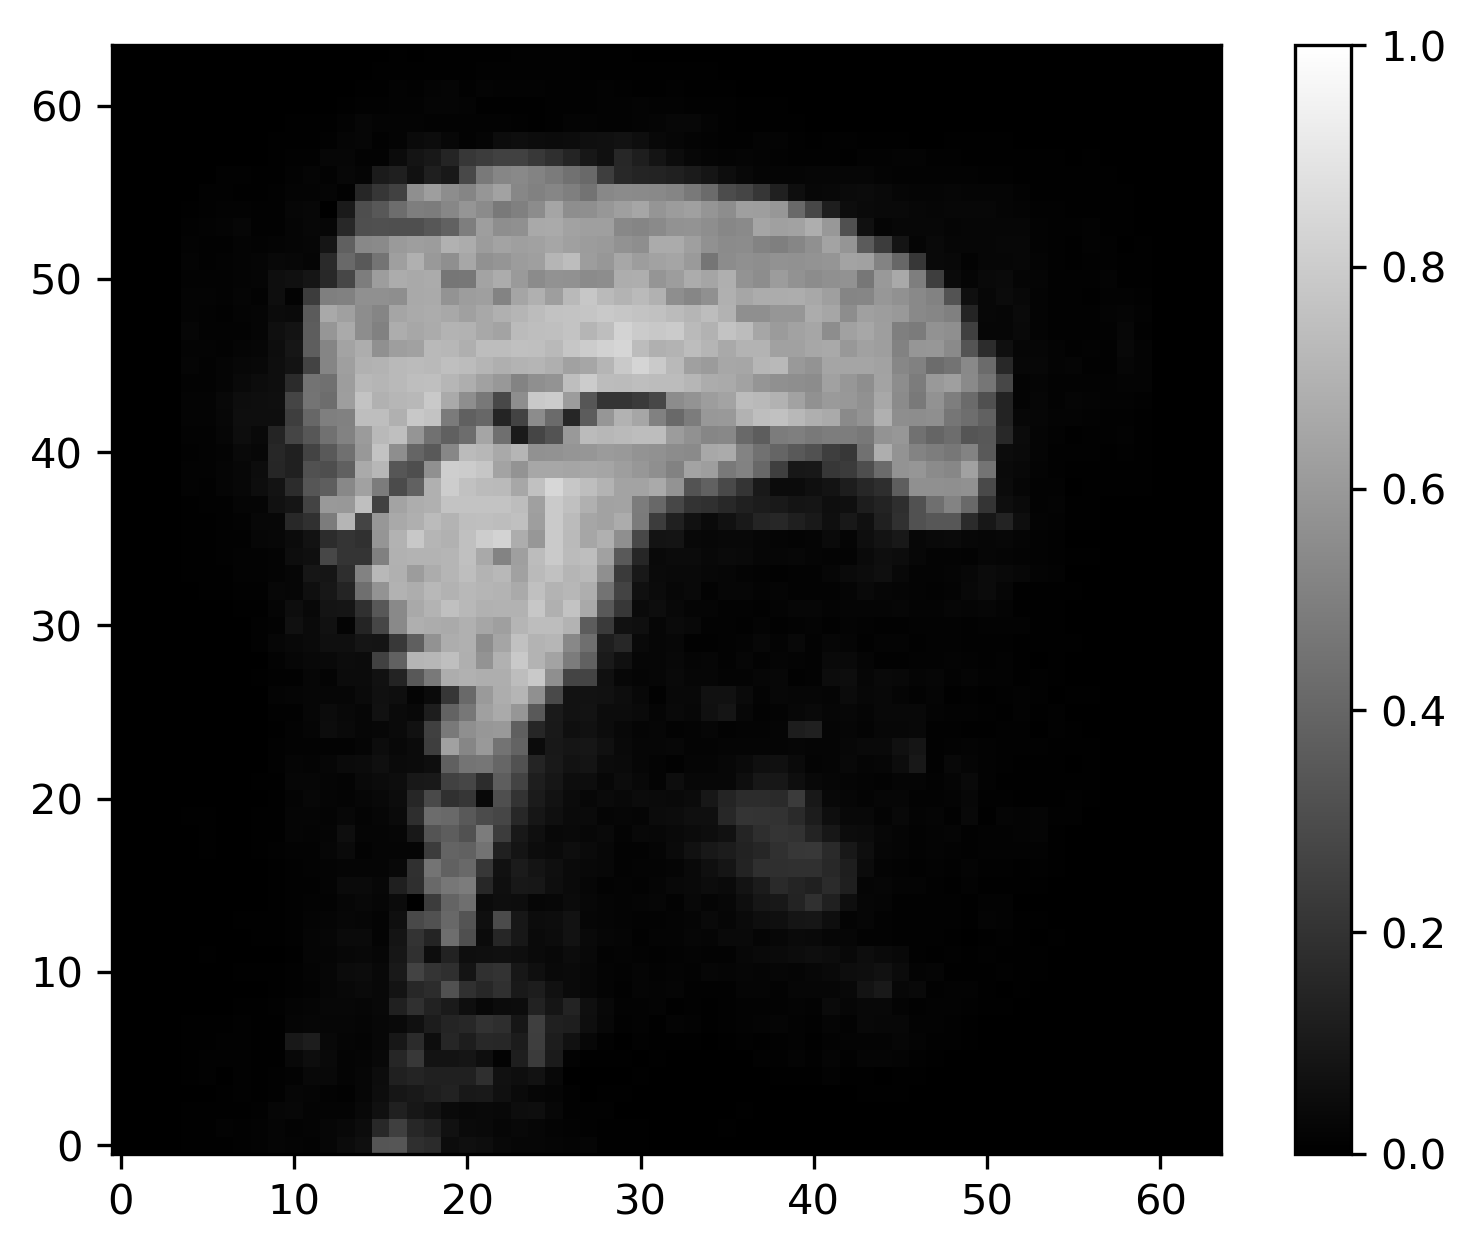
\includegraphics[width=0.33\textwidth]{sub-04-5-1-1000/sub-04-5-1-1000-100-20-_-_-test.png}}}
		\hfill
		\subfloat[Восстановленный]{\label{fig:4b}{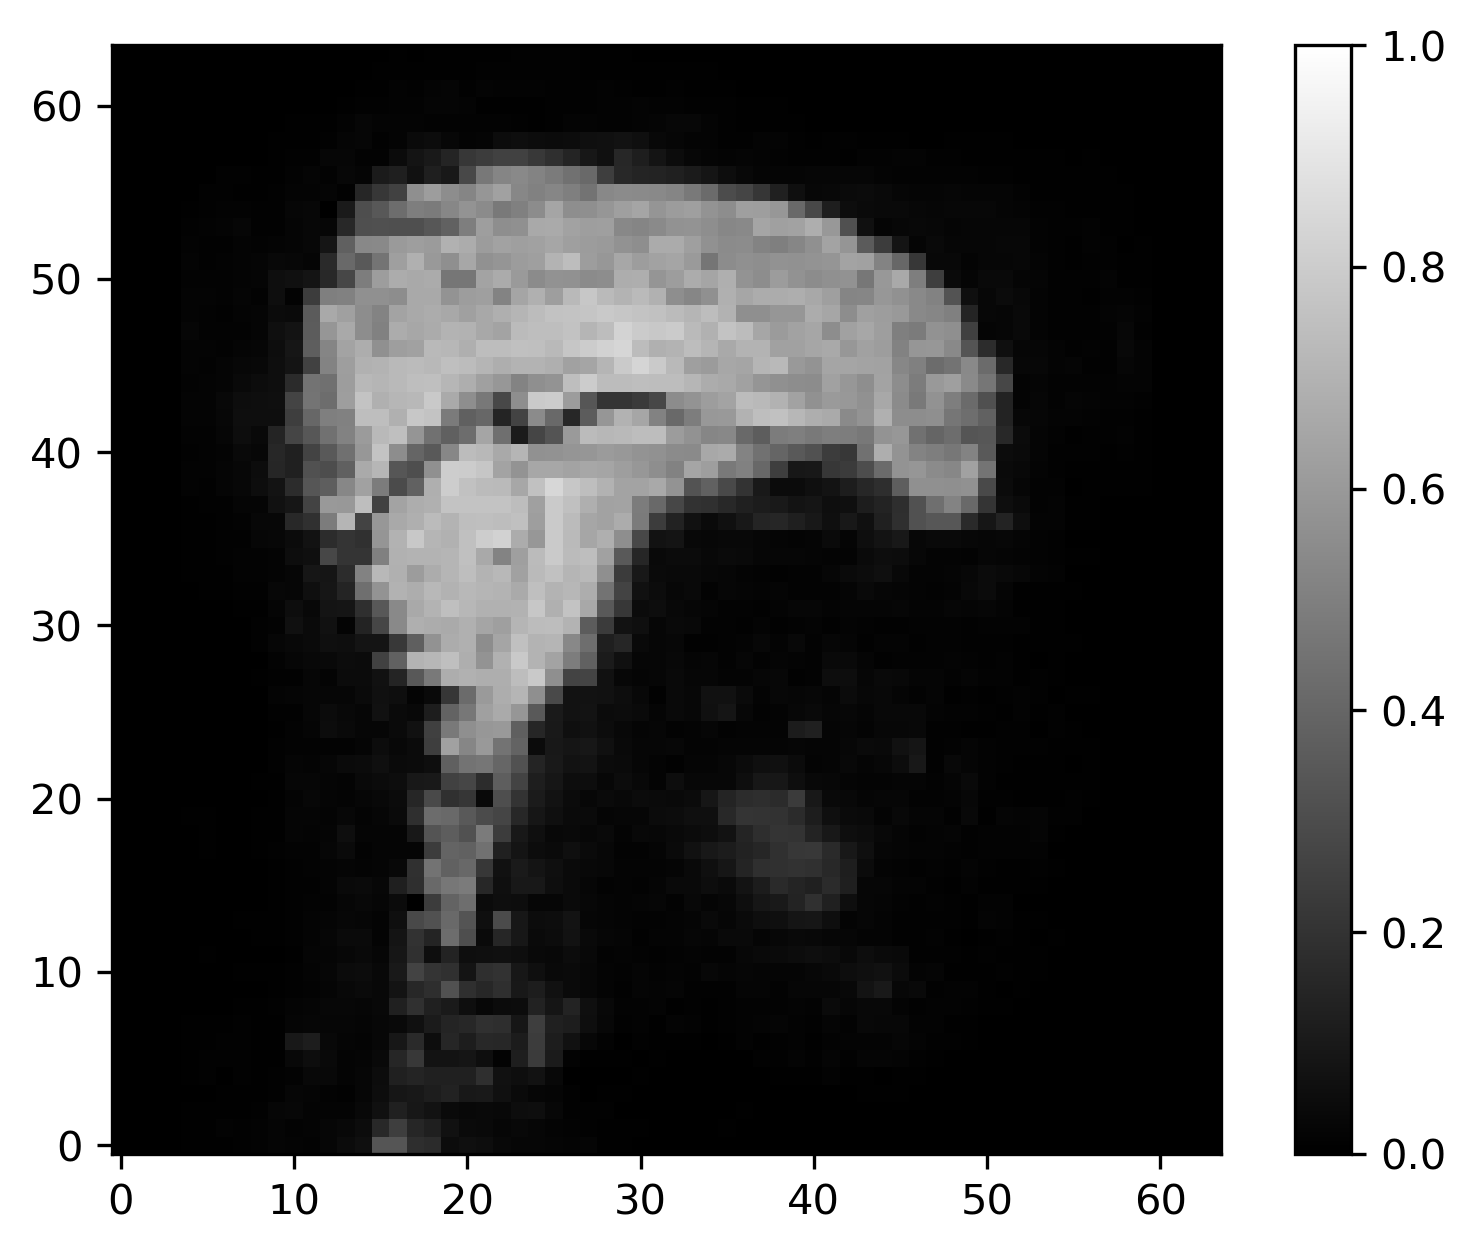
\includegraphics[width=0.33\textwidth]{sub-04-5-1-1000/sub-04-5-1-1000-100-20-_-_-predicted.png}}}
		\hfill
		\subfloat[Разность]{\label{fig:4c}{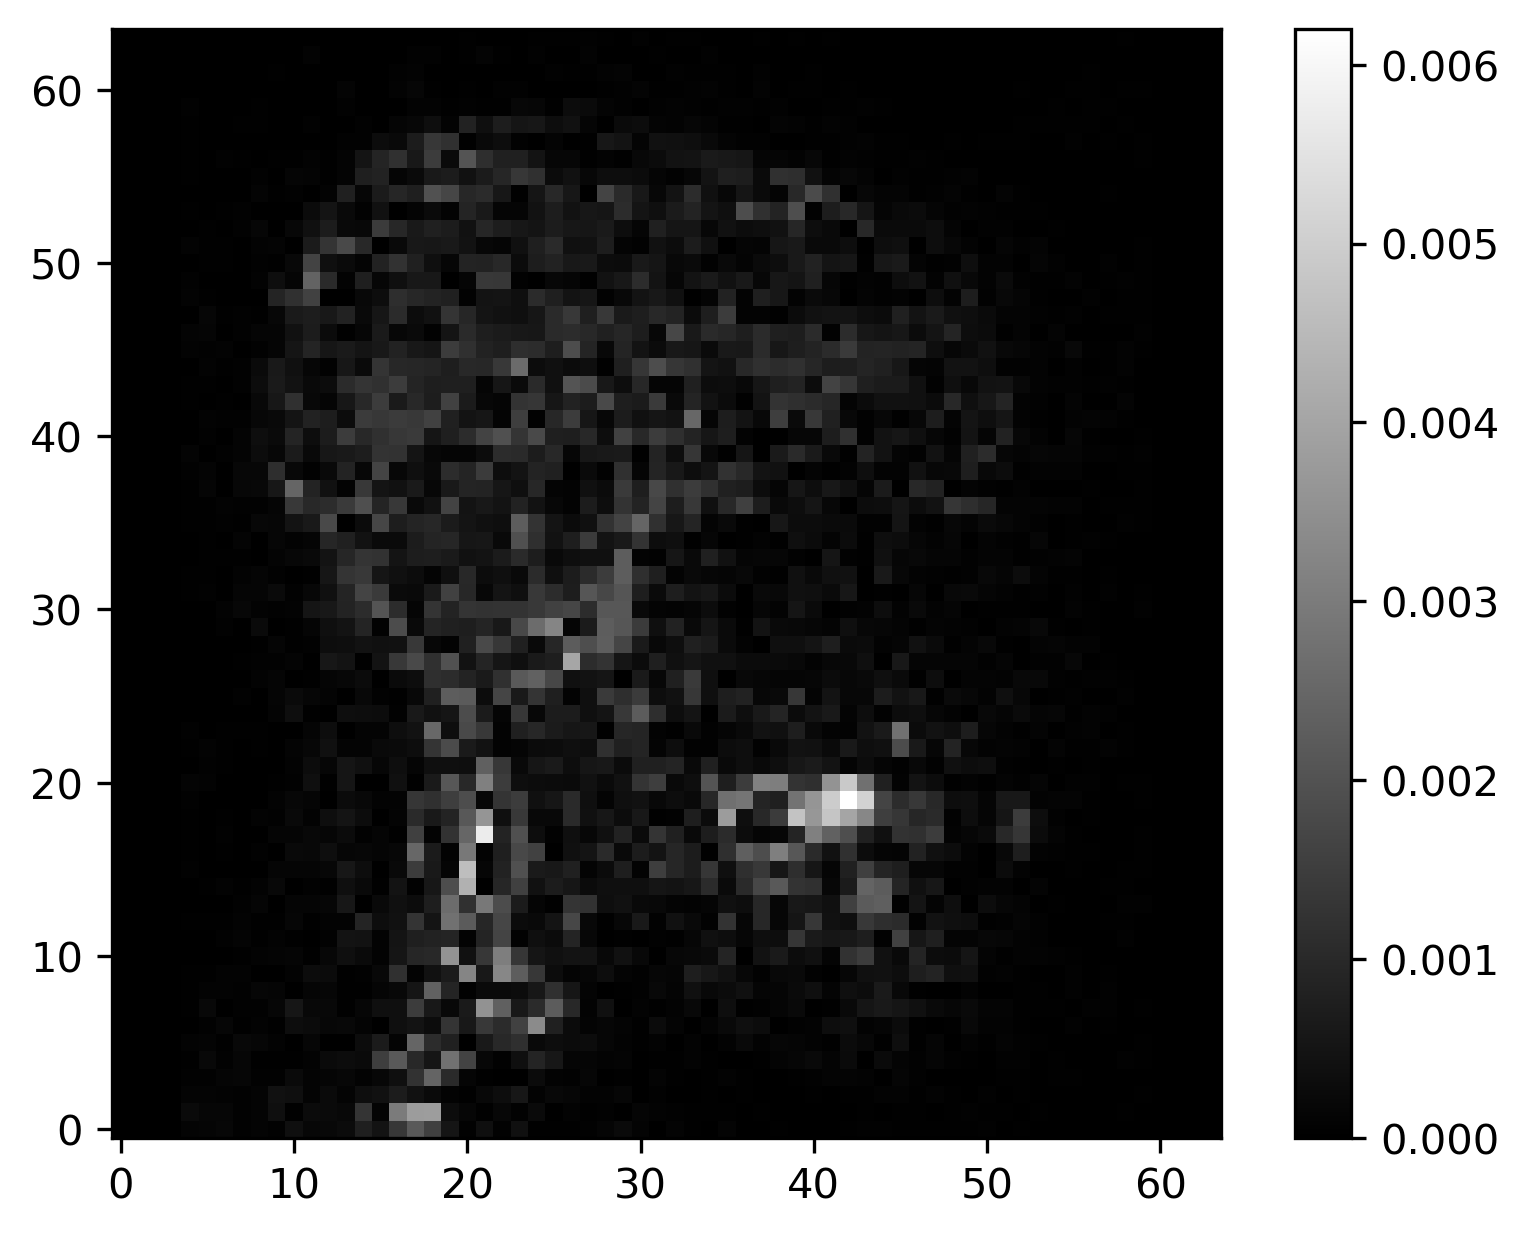
\includegraphics[width=0.33\textwidth]{sub-04-5-1-1000/sub-04-5-1-1000-100-20-_-_-difference.png}}}
		\caption{Срез снимка фМРТ из тестовой выборки}
		\label{fig:4}
	\end{figure}

	Проведен анализ зависимости MSE от коэффициента регуляризации $\alpha$.
	Рассматривались коэффициенты сжатия 1, 2, 4 и 8. 
	Соответствующие графики приведены на Рис.~\ref{fig:5}.
	Из графиков видно, что оптимальное значение коэффициента $\alpha \approx 100$.

	\begin{figure}[h!]
		\centering
		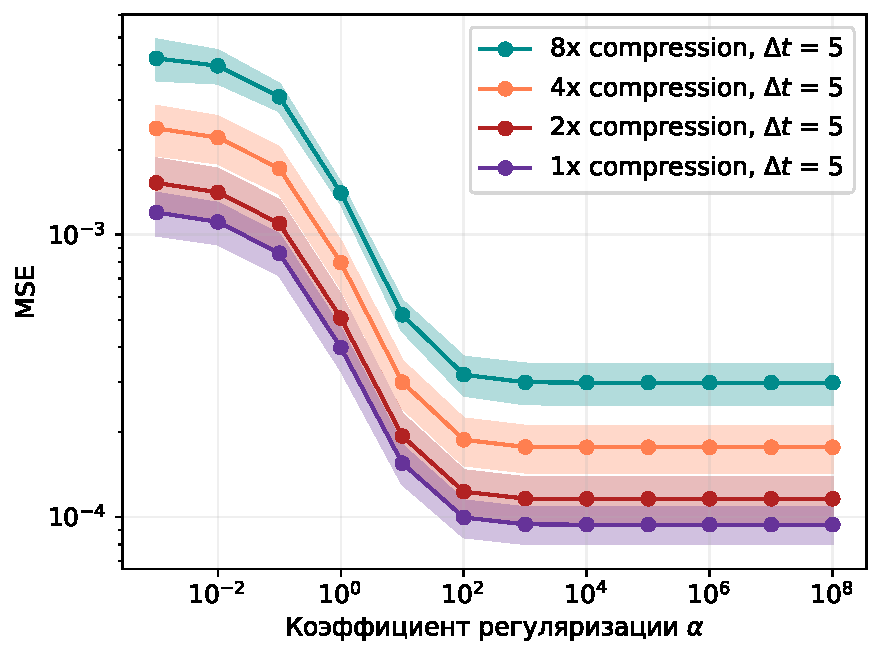
\includegraphics[width=0.65\textwidth]{subs_MSE_alpha.pdf}
		\caption{Зависимость метрики MSE от коэффициента регуляризации $\alpha$ на снимках из тестовой выборки}
		\label{fig:5}
	\end{figure}

	Построен график распределения значений компонент вектора весов модели.
	Для построения производилось усреднение по всем вокселям фиксированного снимка.
	Результат представлен на Рис.~\ref{fig:6}.
	Аппроксимация распределения схожа с плотностью нормального распределения.
	Это может говорить о том, что построенная модель, вероятно, имеет определенную
	статистическую значимость.

	\begin{figure}[h!]
		\centering
		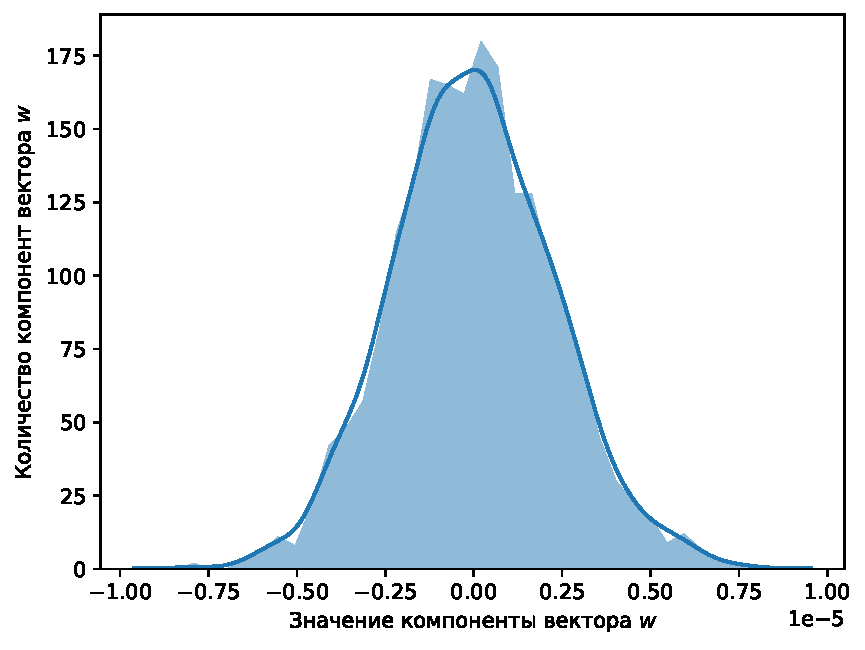
\includegraphics[width=0.65\textwidth]{mean_weight_distribution.pdf}
		\caption{Распределение значений компонент вектора весов}
		\label{fig:6}
	\end{figure}

	Проведена проверка гипотезы инвариантности весов модели относительно человека.
	Другими словами, восстановление снимка фМРТ одного человека можно производить, используя
	матрицу весов другого испытуемого. Использовалась метрика MSE на тестовой выборке.
	Результаты представлены в Таблице~\ref{table:1}.

	\begin{table}[h!]
		\centering
		\begin{tabular}{|c|c|c|}
			\hline
			Матрица весов	&	Истинная	&	Подмешанная \\ \hline \hline
			MSE		& 	$1.02 \cdot 10^{-4}$	 &		$1.05 \cdot 10^{-4}$ \\ \hline
		\end{tabular}
		\caption{Проверка гипотезы инвариантности весов модели относительно человека}
		\label{table:1}
	\end{table}

	Рассмотрено качество работы метода на случайном шуме. В качестве матрицы $\bX$ из \eqref{eq18}
	взята матрица случайных чисел из $[0, 1)$. Произведено сравнение с результатами на настоящей
	выборке. К первому снимку последовательно прибавляются все восстановленные изменения значений
	вокселей. В результате имеем последний снимок последовательности. На Рис.~\ref*{fig:7}
	представлены срезы последнего истинного и восстановленного снимков из тестовой выборки. 
	На Рис.\myfigref{fig:7}{fig:7c} можно наблюдать разность между ними.
	Результаты на случайном шуме продемонстрированы на Рис.~\ref*{fig:8}.
	Можно видеть, что разность между истинным и восстановленным снимками при работе со случайным шумом
	значительно выше. Численные результаты приведены в Таблице~\ref{table:2}.

	\begin{figure}[h!]
		\centering
		\subfloat[Истинный]{\label{fig:7a}{\includegraphics[width=0.33\textwidth]{sub-35-5-1-1000/original/sub-35-5-1-1000--1-20-_-_-recovered-test.png}}}
		\hfill
		\subfloat[Восстановленный]{\label{fig:7b}{\includegraphics[width=0.33\textwidth]{sub-35-5-1-1000/original/sub-35-5-1-1000--1-20-_-_-recovered-predicted.png}}}
		\hfill
		\subfloat[Разность]{\label{fig:7c}{\includegraphics[width=0.33\textwidth]{sub-35-5-1-1000/original/sub-35-5-1-1000--1-20-_-_-recovered-difference.png}}}
		\caption{Срез снимка фМРТ из тестовой выборки}
		\label{fig:7}
	\end{figure}

	\begin{figure}[h!]
		\centering
		\subfloat[Истинный]{\label{fig:8a}{\includegraphics[width=0.33\textwidth]{sub-35-5-1-1000/noised/sub-35-5-1-1000--1-20-_-_-recovered-test.png}}}
		\hfill
		\subfloat[Восстановленный]{\label{fig:8b}{\includegraphics[width=0.33\textwidth]{sub-35-5-1-1000/noised/sub-35-5-1-1000--1-20-_-_-recovered-predicted.png}}}
		\hfill
		\subfloat[Разность]{\label{fig:8c}{\includegraphics[width=0.33\textwidth]{sub-35-5-1-1000/noised/sub-35-5-1-1000--1-20-_-_-recovered-difference.png}}}
		\caption{Срез снимка фМРТ из тестовой выборки (на случайном шуме)}
		\label{fig:8}
	\end{figure}

	\begin{table}[h!]
		\centering
		\begin{tabular}{|c|c|c|}
			\hline
			Выборка	&	Истинная	&	Случайный шум \\ \hline \hline
			MSE		& 	$2 \cdot 10^{-3}$	 &		$10^{-1}$ \\ \hline
		\end{tabular}
		\caption{Качество работы метода на случайном шуме}
		\label{table:2}
	\end{table}

\newpage

\section{Заключение}

	Построен базовый и основной методы восстановления снимков фМРТ по видеоряду, просматриваемому
	человеком. Базовый метод основан на восстановлении следующего снимка по одному изображению.
	В основном методе используется одно изображение и предыдущий снимок фМРТ.
	Оба метода показывают справедливость гипотезы о линейной зависимости между данными.
	Кроме того, продемонстрирована зависимость качества методов от времени задержки.
	Качество работы основного метода значительно лучше.
	Это подтверждает гипотезу о взаимосвязи снимков в последовательности.
	Проверена гипотеза инвариантности весов модели относительно человека.

\newpage

\bibliographystyle{plain}
\bibliography{Kiselev2023fMRI.bib}

\end{document}